\documentclass[conference]{IEEEtran}
\IEEEoverridecommandlockouts
% The preceding line is only needed to identify funding in the first footnote. If that is unneeded, please comment it out.
\usepackage{tabularx}
\usepackage{booktabs}
\usepackage{cite}
\usepackage{amsmath,amssymb,amsfonts}
\usepackage{algorithmic}
\usepackage{graphicx}
\usepackage{textcomp}
\usepackage{xcolor}
\usepackage{listings}
\lstset{basicstyle=\ttfamily,
  showstringspaces=false,
  commentstyle=\color{red},
  keywordstyle=\color{blue}
}
\def\BibTeX{{\rm B\kern-.05em{\sc i\kern-.025em b}\kern-.08em
    T\kern-.1667em\lower.7ex\hbox{E}\kern-.125emX}}
\begin{document}

\title{Applied Deep Learning Final Project\\}

\author{\IEEEauthorblockN{1\textsuperscript{st} Noah Campise}
\IEEEauthorblockA{\textit{Applied Deep Learning} \\
Lakeland, Fl \\
ncampise2655@floridapoly.edu}
}

\maketitle

\section{Introduction}
This is the report for the Applied Deep Learning final project. For this project, I fine-tuned the Uncased Base BERT Language Model (\cite{bert_paper}) on the ISOT datset in order to create a Fake news detector.

\subsection{Motivation}
We live in a world entangled in the digital technologies that facilitate our every day lives. These technologies have allowed for an information explosion. Part of the information landscape is the set of news articles that can inform our decisions in impactful ways. 

The empowerment of information technologoes to spread true information is vulnerable to explotation to spread misinformation.  Part of this misinformation is Fake news, which can hurt the decision making of everyday people, since they may not have the time to review what they are reading. Furthermore, Fake news is especially dubious misinformation, since it can break people's trust in actual, informative news.

\subsection{Problem}

In the information landscape, there is a considerable amount of Fake news that can misinform people, resulting in them making decisions against interests of themselves and their communities.

\subsection{Solution}

This report details the training of a Nueral Network capable of detecting Fake news from True news, which will help people to filter out these false news articles.

\section{Dataset}

In order to fine-tune the BERT model, I need to process the data in a way that is BERT native.


\subsection{ISOT Dataset}

The ISOT dataset (\cite{isot_dataset}) contains over 37,000 articles of true and fake news. It is used to fine-tune the BERT model in order to for it to be a good fake-news detector.

This dataset is broken into True.csv and Fake.csv, for true and fake news respectively. Each csv has the following columns:

\begin{itemize}
  \item title: Title of a given article
  \item text: Article text
  \item subject: Article subject
  \item date: Article date
\end{itemize}

\subsection{Benefits to using the ISOT dataset}

There is less fake news that real news, which would result in a skewed dataset. If one were to randomly sample from this set and train a model, the model would learn just to predict that every article is real news, instead of having to learn real news from fake news.

The ISOT dataset is a near 50/50 split between fake and real news. This means that the model will have to look for the differences between real and fake articles. 

\subsection{Data Cleaning}

We removed the subject and date columns during this project. This is because the subject field might be a giveaway to the model and giveaway whether or not the article is True or Fake. The date field should have no relation on whether or not an article is True or Fake.

\subsection{BERT Native Changes}


Furthermore, the ISOT dataset provides both the Title and the Text in seperate columns. This means that it is easy to use a BERT native seperator token between the columns. BERT was pre-trained using the seperator tokens in order to weigh the importance of the title differently than that of the text.

\subsection{Training, Validation, and Testing}

In order to create the sets used for training, validation, and testing, we will use the train\_test\_split twice in order to create these sets. Furthermore, we use the stratify\_by\_column parmaeter to ensure that there is an even spread of Fake and True entries between sets.

This is implemented in the code seen in \ref{lst:tvt-sets}. First, I create a train and test split of 80-20. From here, I create a further split of the test set into a test and validation set of 50-50. Creating a traing, test, and validation split of 80-10-10. 

I also set the stratify\_by\_column to the label column. This way, articles of Fake and True news are split evenly among each set.

These sets are then combined into one DatasetDict. This is a transformers library native data type that allows for an easy integration between the data and the training pipeline.


\begin{lstlisting}[language=Python,caption={Training, Validation, and Testing Sets},label={lst:tvt-sets}]
ds = Dataset.from_pandas(df)

ds = ds.class_encode_column("label")

train_remainder_split =
  ds.train_test_split(
    test_size=0.2, 
    seed=42, 
    stratify_by_column="label"
  )

test_val_split =
  train_remainder_split['test']
    .train_test_split(
      test_size=0.5,
      seed=42,
      stratify_by_column="label"
    )

# Combine into a single DatasetDict
from datasets import DatasetDict

split_dataset = DatasetDict({
    'train':
      train_remainder_split['train'],
    'test':
      test_val_split['test'],
    'validation':
      test_val_split['train']
})
\end{lstlisting}

\section{Methodology}

For this project, I fine-tuned the bert-base-uncased model using python libraries pandas, transformers, and datasets.

\subsection{Tokenize datasets}

The implementation of dataset tokenization can be seen in \ref{lst:ds-token}

In order to get the dataset in a BERT native format, we need to tokenize the datasets. This is acheived using the Autotokenizer form the bert-base-uncased.

We use uncased since there may be inconsistent capitalization between True and Fake news articles, which it would be safer to ignore that difference.

Furthermore, the title and text columns are tokenized as different sections, which BERT can distinguish between the two.

Furthermore, the tokenizer uses a padding of max\_length so that any article shorter than the max length will have padding tokens to fit the max size in a batch.

For any article large than the limit, the model will cut off the rest in order to prevent Out of Memory Errors on my RTX 4070.

The max\_length is set to 256 to balance VRAM usage on RTX 4070


\begin{lstlisting}[language=Python,caption={Dataset Tokenization},label={lst:ds-token}]
from transformers import AutoTokenizer

tokenizer = AutoTokenizer
  .from_pretrained("bert-base-uncased")

def tokenize_function(examples):
    return tokenizer(
        examples["title"], 
        examples["text"], 
        padding="max_length", 
        truncation=True, 
        max_length=256
    )

tokenized_datasets = split_dataset.map(
  tokenize_function,
  batched=True
)
\end{lstlisting}


\subsection{Model selection}

The code implementation of the model can be seen in the code \ref{lst:model-sel}

For this project, I chose the bert-base-uncased in order to stick to remote the potential connections between capitalization and the prediction. 

I use the id2label and label2id in order to map between 0 and 1 and Fake and True.

\begin{lstlisting}[language=Python,caption={Model Selection},label={lst:model-sel}]
id2label = {0: "FAKE", 1: "TRUE"}
label2id = {"FAKE": 0, "TRUE": 1}

model_name = "bert-base-uncased"
model = AutoModelForSequenceClassification
  .from_pretrained(
    model_name,
    num_labels=2,
    id2label=id2label,
    label2id=label2id
  )
\end{lstlisting}

\subsection{Training Parameters.}

Some parameters to to take note of, the batch size per GPU is set to 16 for training and evaluation, since I am training on my own hardware and need to ensure that I am not using all of the my resources when training. 

I set the learning rate to a 5e-5, so that there is no overstepping.

The model is set to train over 20 epochs to ensure that the prediction is able to approach a high accuracy. 

The metric for training is f1, since this accounts for both recall and precision, which a balance between both is required for a model that detects fake news. This metric is set so that the higher the f1 score, the better the model.

Also, instead of using fp16 precision, I set it to use bp16, which is native to my GPU's architecture.

These arguments are set using the code in \ref{lst:traing_args}, which is based on the work in \cite{medium_bert_guide}.

\begin{lstlisting}[language=Python,caption={Training Arguments},label={lst:traing_args}]
from transformers import TrainingArguments

# Define training arguments
training_args = TrainingArguments(
    output_dir="./results",           
    eval_strategy="epoch",     
    learning_rate=5e-5,              
    per_device_train_batch_size=16,  
    per_device_eval_batch_size=16,
    num_train_epochs=20,              
    weight_decay=0.01,               
    save_total_limit=2,              
    load_best_model_at_end=True,     
    metric_for_best_model="f1",      
    greater_is_better=True,          
    
    logging_steps=100,               
    bf16=True,                        
    save_strategy="best"
)

print(training_args)
\end{lstlisting}

\subsection{Compute metrics}

The compute\_metrics function computes both the f1 and accuracy score of the model when evaluating.

The reason that I chose to calculate both the f1 and accuracy is to create a metric that the training pipeline will try to maximize (f1) and a metric that is easy to understand (accuracy). 

The by training the model to have a high f1 score, we are training the model to balance both the precision and the recall, which will help to build a model resilient to data imbalances between the True and Fake news articles.

The code in \ref{lst:compute-metrics} is used by the transformers library to calculate both the f1 score and the accuracy. For calculating the f1 score, I set the average parameter to weighted, since this will calculate f1 for predictions on both True and Fake news articles.

\begin{lstlisting}[language=Python,caption={Compute Metrics},label={lst:compute-metrics}]
metric_f1 = load("f1")
metric_acc = load("accuracy")
def compute_metrics(eval_pred):
    logits, labels = eval_pred
    predictions = logits.argmax(axis=-1)

    f1  = metric_f1.compute(
      predictions=predictions,
      references=labels,
      average="weighted"
    )
    acc = metric_acc.compute(
      predictions=predictions,
      references=labels
    )
    return {**f1, **acc}
\end{lstlisting}

\section{Results and Discussion}

This section is used to discuss the results of the fine-tuned model after training it over 20 epochs.

Our validation f1 score can be seen overtime in the table \ref{fig:epoch-valid} The f1 score can be seen at a peak of .921 and an accuracy of .921 at epoch 17.

Overall, we can see that this model is capable of accurately predicting Fake news from True news.

\begin{figure}[ht] % [h] forces the image to be placed 'here'
    \centering
    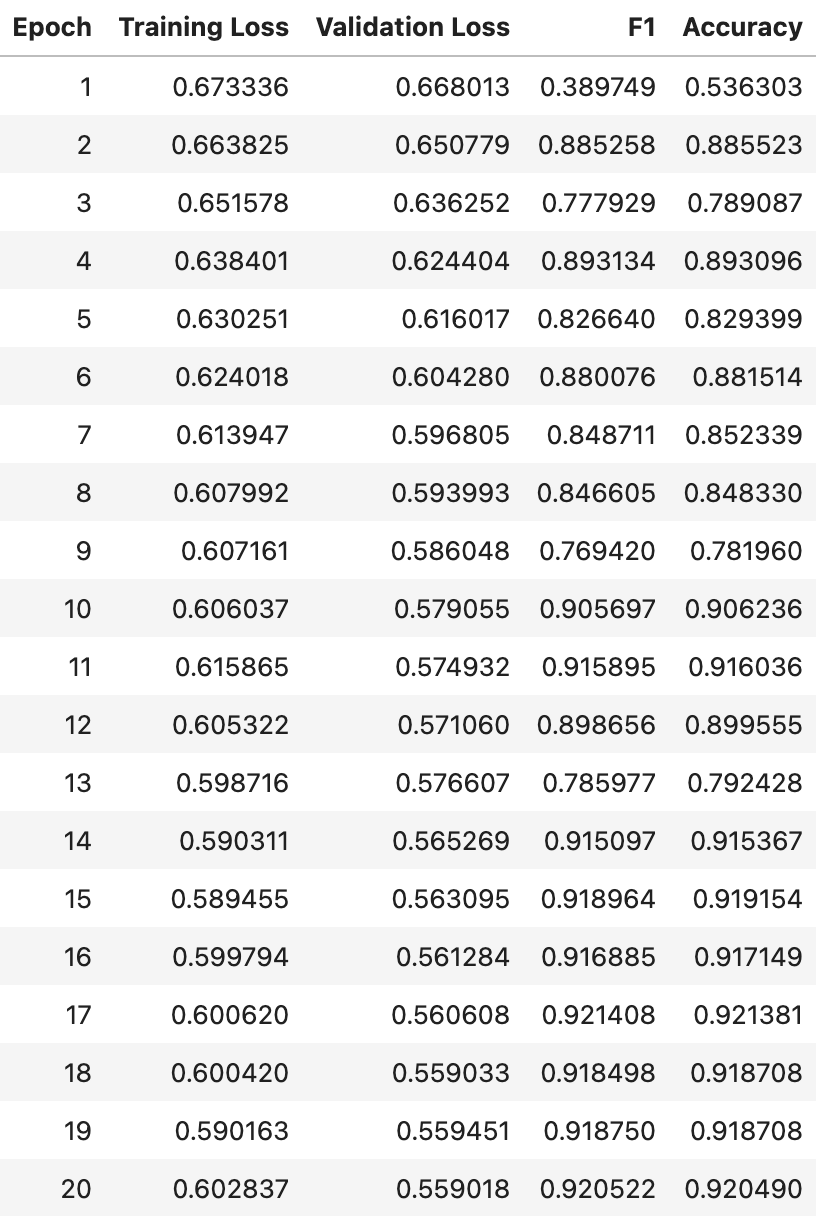
\includegraphics[width=0.5\textwidth]{epoch-valid.png}
    \caption{Table of metrics over epochs}
    \label{fig:epoch-valid}
\end{figure}

\subsection{F1 and Accuracy overtime}

The image \ref{fig:f1_over_epoch} Accuracy and F1 score of the validation set over each training epoch. This shows us that after training on 14 epochs, the model's performance stagnates.


\begin{figure}[ht] % [h] forces the image to be placed 'here'
    \centering
    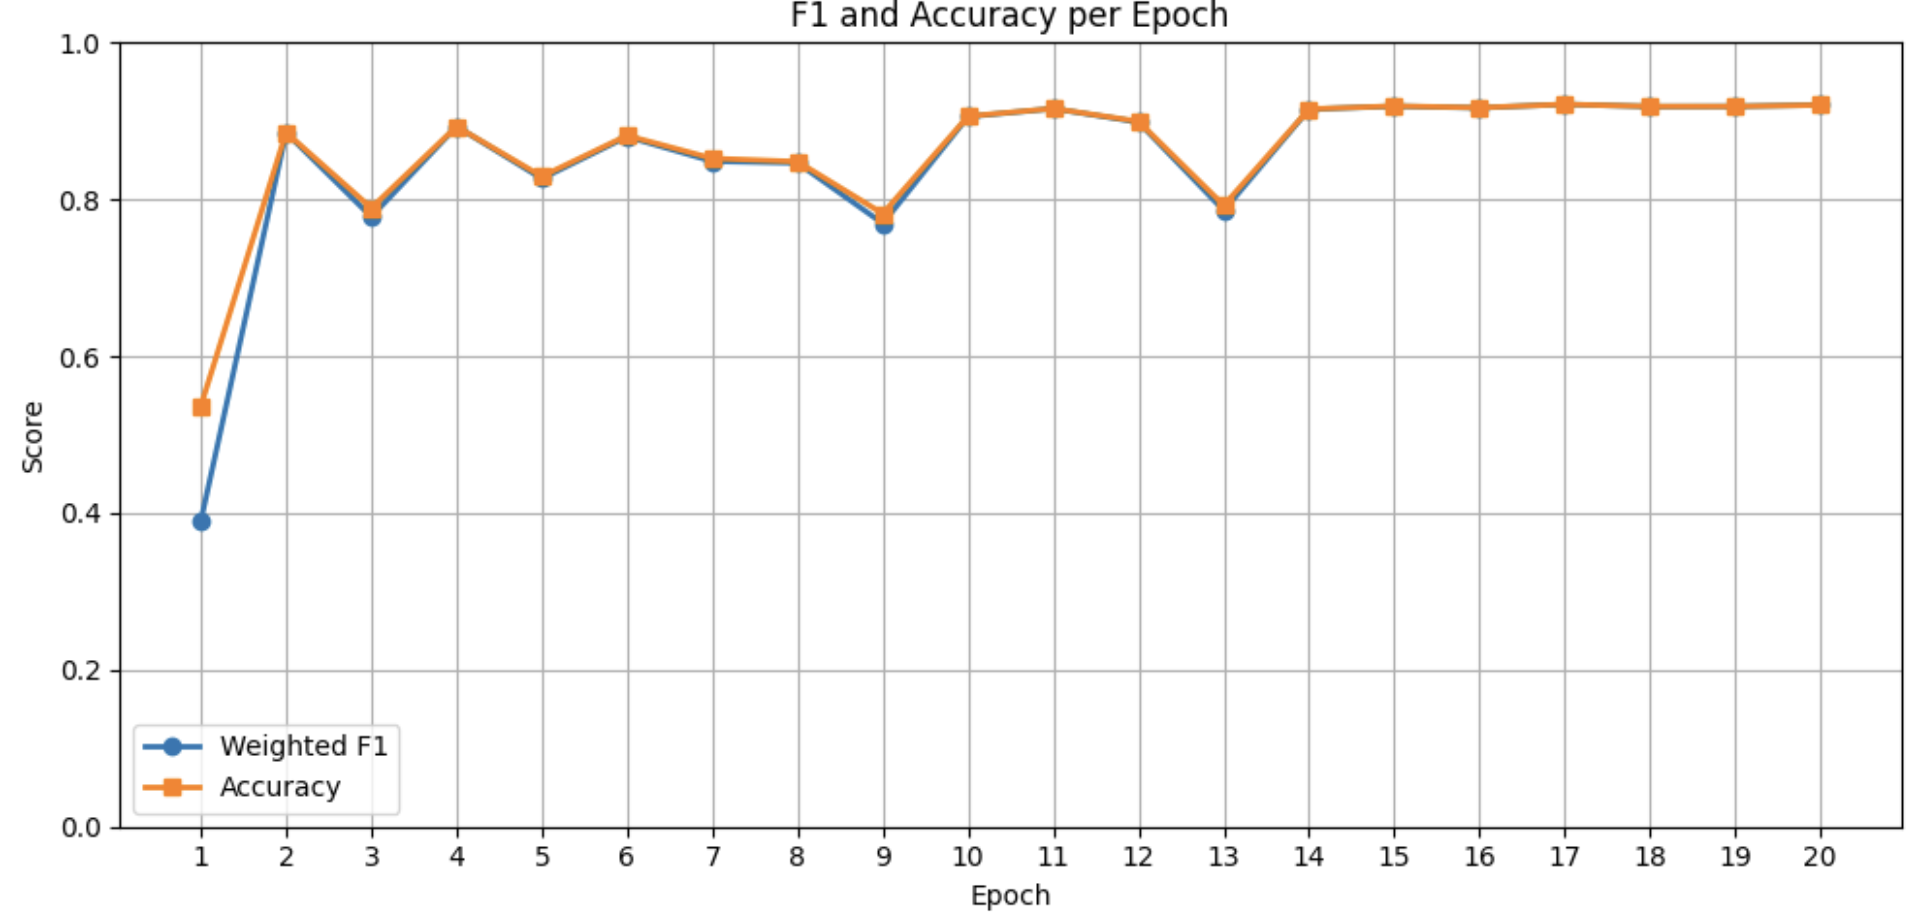
\includegraphics[width=0.5\textwidth]{f1-over-epoch.png}
    \caption{F1 Score and Accuracy over time}
    \label{fig:f1_over_epoch}
\end{figure}

\subsection{Accuracy, F1 Score, and Confusion Matrix}

We can see that in the confusion matrix \ref{fig:confusion_matrix}, that the model is more likely to predict Fake news as True than it is to predict True news as Fake.

\begin{figure}[ht] % [h] forces the image to be placed 'here'
    \centering
    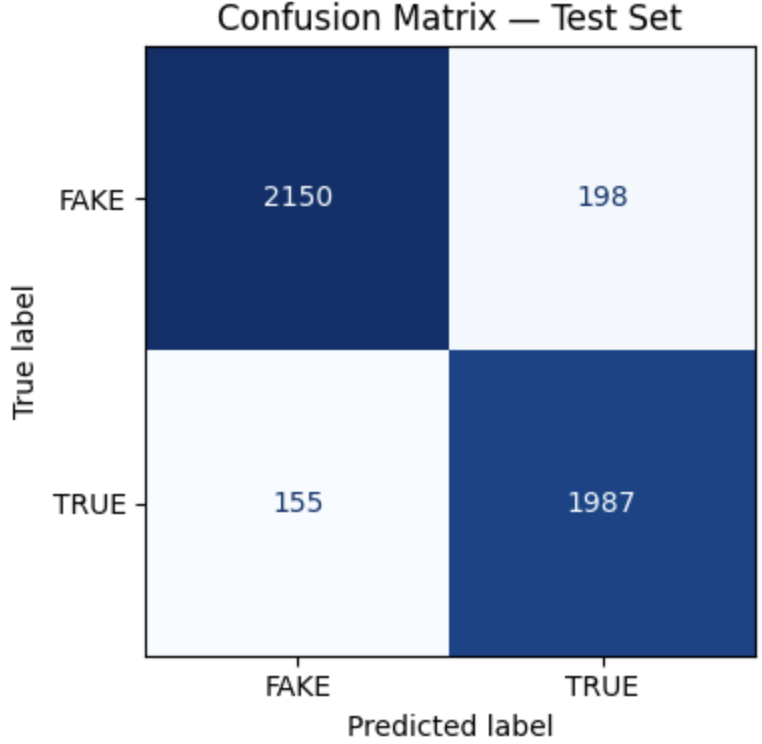
\includegraphics[width=0.5\textwidth]{confusion.png}
    \caption{Confusion Matrix for Fake News Detection}
    \label{fig:confusion_matrix}
\end{figure}

\subsection{Qualitative Analysis}

The table \ref{tab:predictions} can be used for qualitative analysis of the model. As we can see, there is a spread in model confidence in the correct predictions between .551 and .872 while for incorrect predictions, the models confidence is below .568. This indicates to us that there is a correlation between confidence and the correct preditions.



\begin{table}[ht]
\centering
\caption{Sample Model Predictions (Qualitative Analysis)}
\label{tab:predictions}
\footnotesize % Smaller font size to fit the column width
\begin{tabularx}{\columnwidth}{X c c r} % Uses columnwidth for half-page/2-col
\toprule
\textbf{Article Title Snippet} & \textbf{True} & \textbf{Pred} & \textbf{Conf.} \\ \midrule
\textit{Correctly Classified} & & & \\ \midrule
Trump Lashes Out At FBI... & FAKE & FAKE & 55.1\% \\
U.S. to continue supporting... & REAL & REAL & 61.7\% \\
Hillary Video Does NOT Want... & FAKE & FAKE & 87.2\% \\
GOP Rep. Jim Jordan Tells... & FAKE & FAKE & 61.8\% \\
UK LEADER: Nothing on Earth... & FAKE & FAKE & 80.9\% \\ \midrule
\textit{Misclassified} & & & \\ \midrule
Bombardier dispute risks... & REAL & FAKE & 51.5\% \\
Republicans Threaten Students... & FAKE & REAL & 53.2\% \\
Trump congratulates China... & REAL & FAKE & 50.8\% \\
College Receives \$280M... & FAKE & REAL & 53.5\% \\
Mueller Team Uniform?... & FAKE & REAL & 56.8\% \\ \bottomrule
\end{tabularx}
\end{table}

\section{Conlusion}
In conclusion, I was able to create an accurate Fake-news detector using the BERT model. This model is able to identify fake news with an accuracy of .921. 

Some of the takeaways is that through natural language processing, we are able to create a model that will accurately detect fake news articles based on their language. 

For future work, one can take this model, and train the BERT model with a few unfrozen layers in order to create a more accurate model. One could also add additional layers using the pytorch library that can identify more complex patterns in the contextual embeddings created by BERT.

\bibliography{references}   % Points to your references.bib file (do not include the .bib extension)
\bibliographystyle{ieeetr} % or 'apa' depending on your project requirements

\end{document}
